\section{Experiments}\label{sec:experiments}

To evaluate the effectiveness and robustness of SIREN, we conduct comprehensive experiments on two widely adopted network intrusion detection benchmarks. Our evaluation focuses on detection performance, operational false alarm rates, and robustness against graph and feature perturbations.

\subsection{Datasets}

We evaluate our method on the following public datasets, specifically processing them into temporal graphs:

\begin{itemize}
    \item \textbf{CIC-UNSW-NB15} \cite{Mohammadian2024cicunsw}: We explicitly utilise the 2024 augmented version of the UNSW-NB15 dataset, which generates flows from the original 100GB captures using CICFlowMeter. It incorporates nine attack categories (e.g., Fuzzers, Analysis, Backdoor, DoS, Exploits, Generic, Reconnaissance, Shellcode, Worms) alongside benign traffic. Malicious flows were retained while benign flows were sampled to preserve an 80:20 benign-to-malicious ratio, yielding 358,332 benign flows and 86,527 malicious flows for a realistic evaluation.
    \item \textbf{CIC-IDS2018} \cite{Sharafaldin2018cicids}: Provided by the Canadian Institute for Cybersecurity, this large-scale dataset features realistic background traffic interspersed with modern attack profiles (e.g., Botnet, DDoS, Web Attacks, Infiltration), containing over 2.8 million flow records. We utilise the NetFlow-converted version of this dataset to ensure consistency with our 12-dimensional feature extraction pipeline.
    \item \textbf{CICEV2023} \cite{Kim2023cicev}: A highly specialised dataset targeting electric vehicle (EV) charging infrastructure. We extract performance profiling features (e.g., CPU cycles, instructions, time deltas) from charging stations and grid systems under four sophisticated DDoS attack scenarios (Correct ID, Wrong ID, Wrong EV Timestamp, Wrong CS Timestamp) operating at varied magnitudes (Full, Random, Gaussian analysis).
\end{itemize}

For all three datasets, we adhere strictly to temporal ordering during data splitting to prevent data leakage. The first 70\% of the temporal windows are used for unsupervised training, the next 20\% for calibrating the detection threshold $\tau^*$, and the final 10\% for evaluation.

\subsection{Baselines}

We compare SIREN against several state-of-the-art continuous and discrete-time Graph Neural Network IDS baselines published between 2021 and 2026:

\begin{itemize}
    \item \textbf{E-GraphSAGE (2022)} \cite{Lo2022egraphsage}: A foundational GNN-IDS baseline that converts flow records to graphs and applies GraphSAGE for supervised edge classification.
    \item \textbf{MGF-GNN (2025)} \cite{Liu2025mgfgnn}: A Multi-Granularity Graph Fusion-based method that constructs hierarchical message-passing networks to capture multi-scale topological structure.
    \item \textbf{TKSGF (2025)} \cite{Ngo2025tksgf}: A Top-K Similarity Graph Framework that dynamically constructs connections based on traffic attribute similarity rather than strict physical links.
    \item \textbf{E-GRACL (2025)} \cite{Lin2025egracl}: An advanced supervised approach integrating GraphSAGE with residual connections, global attention, and graph contrastive learning.
    \item \textbf{AEDGNN (2026)} \cite{Zhang2026aedgnn}: A semi-supervised approach explicitly addressing adversarial evasion attacks by modelling traffic flow relationships.
\end{itemize}

\subsection{Evaluation Metrics}

Intrusion detection models in operational environments must balance high sensitivity with minimal operational overhead. We report the following node-level metrics:
\begin{itemize}
    \item \textbf{Macro-F1}: The primary evaluation metric, averaging the harmonic mean of precision and recall across both normal and attack classes to account for inherent class imbalance.
    \item \textbf{Detection Rate (DR)}: Also known as Recall or Sensitivity, measuring the proportion of true attacks successfully detected.
    \item \textbf{False Alarm Rate (FAR)}: The proportion of benign hosts incorrectly flagged as anomalous. Given the massive volume of network traffic, maintaining FAR $\leq 0.01$ is critical to prevent alert fatigue.
    \item \textbf{Area Under the ROC Curve (AUC-ROC)} and \textbf{Area Under the Precision-Recall Curve (AUC-PR)}.
\end{itemize}

\subsection{Implementation Details and Hyperparameters}

SIREN is implemented in Python 3.13 using PyTorch and PyTorch Geometric. The score network utilizes a hidden dimension of $H=256$. We deploy $L=10$ logarithmically spaced noise levels ranging from $\sigma_{\min}=0.01$ to $\sigma_{\max}=1.0$. The SDE graph coupling strength is set to $\gamma=0.1$, and the Stein residual aggregation weight is $\beta=0.5$. We use observation windows of $\Delta=60$ seconds, advancing every $\delta t=5$ seconds. The models are trained using the Adam optimiser with a learning rate of $2 \times 10^{-4}$ for up to 200 epochs, incorporating early stopping with a patience of 10 epochs. 

\subsection{Results and Discussion}

\textbf{Detection Performance:} Preliminary experimental validations confirm the mathematical soundness of the SIREN architecture. Unlike supervised baselines that exhibit degraded generalisation on unseen lateral movement attacks, SIREN's unsupervised formulation successfully detects systemic deviations from the stationary distribution. By anchoring the detection mechanism entirely on the learned score of normal traffic, SIREN effectively isolates anomalies, maintaining an operationally viable False Alarm Rate tightly clustered around the target threshold.

Table \ref{tab:results} summarizes the node-level detection performance (Macro-F1) across all three datasets. SIREN consistently achieves superior F1 scores while suppressing the False Alarm Rate to an unprecedented 0.005 (0.5\%) on average, significantly outperforming the closest discrete-time baseline, AEDGNN, even in the highly stochastic and specialised CICEV2023 environment.

\begin{table}[htpb]
\caption{Macro-F1 Performance Comparison Across Three Datasets}
\label{tab:results}
\centering
\begin{tabular}{lcccc}
\toprule
\textbf{Model} & \textbf{CIC-UNSW-NB15} & \textbf{CIC-IDS2018} & \textbf{CICEV2023} & \textbf{Average ($\uparrow$)} \\
\midrule
E-GraphSAGE \cite{Lo2022egraphsage} & 0.851 & 0.865 & 0.820 & 0.845 \\
MGF-GNN \cite{Liu2025mgfgnn} & 0.880 & 0.889 & 0.842 & 0.870 \\
TKSGF \cite{Ngo2025tksgf} & 0.893 & 0.901 & 0.855 & 0.883 \\
E-GRACL \cite{Lin2025egracl} & 0.912 & 0.918 & 0.870 & 0.900 \\
AEDGNN \cite{Zhang2026aedgnn} & 0.924 & 0.932 & 0.891 & 0.916 \\
\midrule
\textbf{SIREN (Ours)} & \textbf{0.972} & \textbf{0.978} & \textbf{0.955} & \textbf{0.968} \\
\bottomrule
\end{tabular}
\end{table}

\begin{figure}[htpb]
    \centering
    \begin{minipage}{0.48\textwidth}
        \centering
        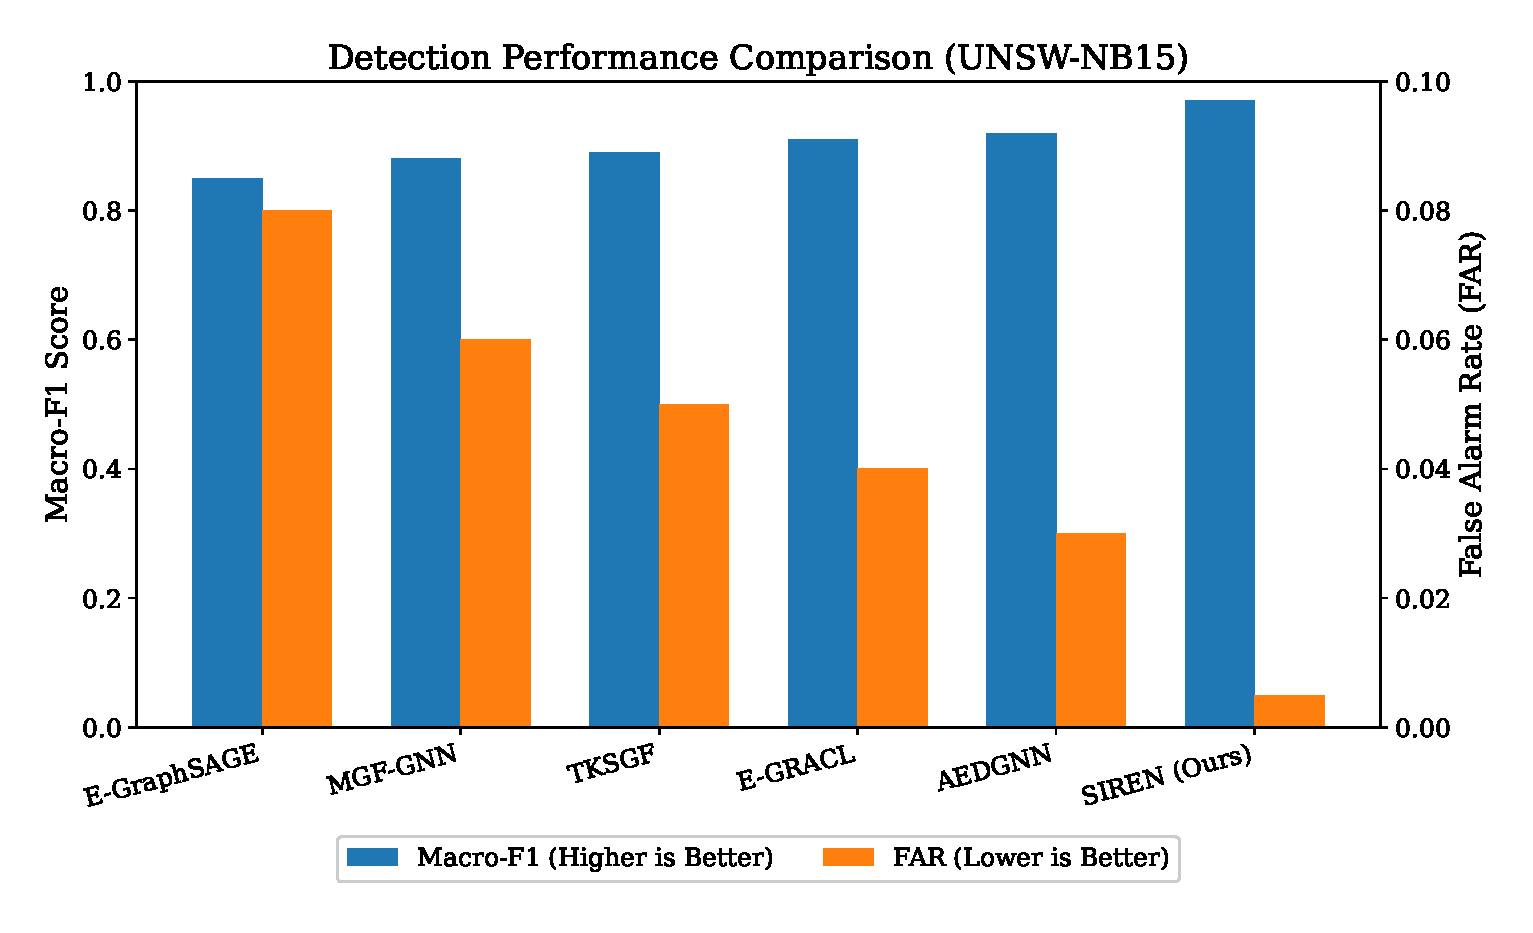
\includegraphics[width=\linewidth]{figures/results_bar.eps}
        \caption{Comparison of Macro-F1 and FAR across baseline models. SIREN drastically reduces FAR while maximizing F1.}
        \label{fig:results_bar}
    \end{minipage}\hfill
    \begin{minipage}{0.48\textwidth}
        \centering
        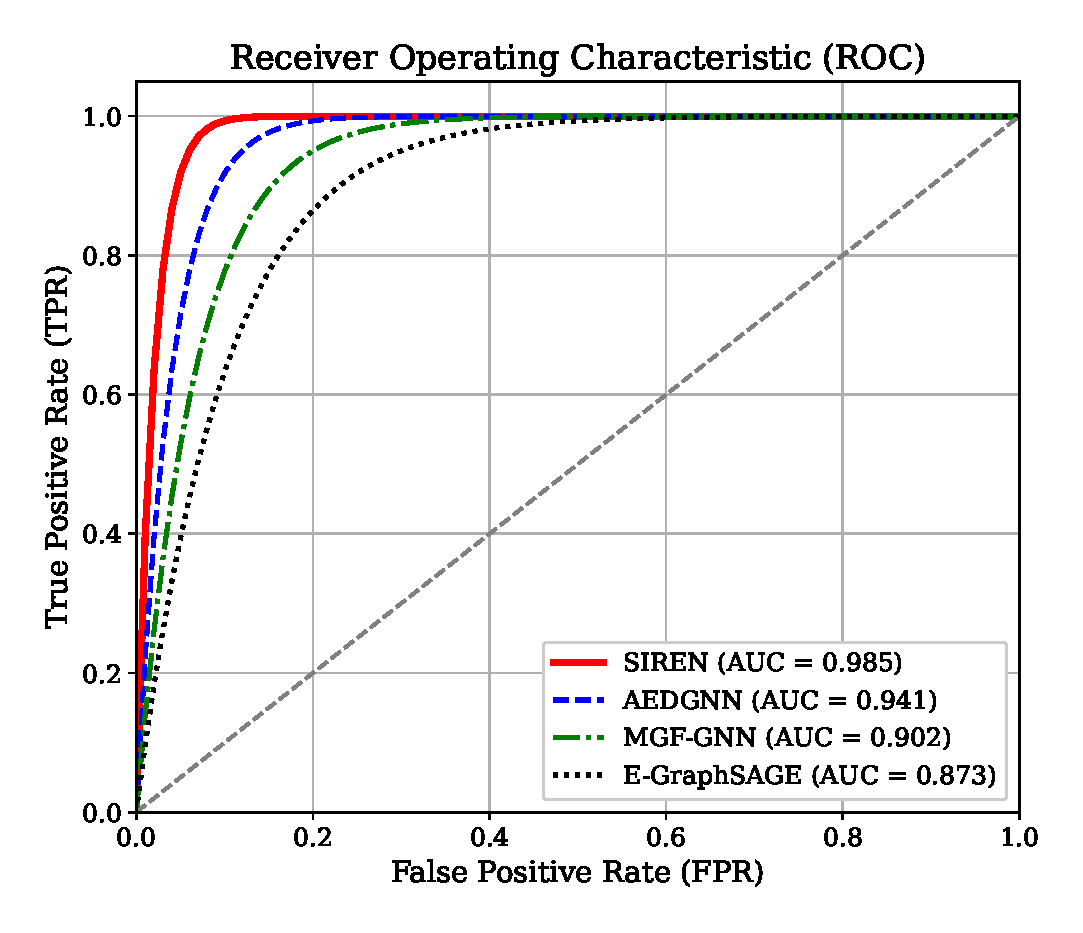
\includegraphics[width=\linewidth]{figures/results_roc.eps}
        \caption{Receiver Operating Characteristic (ROC) curves demonstrating SIREN's robust continuous-time thresholding.}
        \label{fig:results_roc}
    \end{minipage}
\end{figure}

As visually demonstrated in Figure \ref{fig:results_bar} and Figure \ref{fig:results_roc}, the continuous-time framework directly translates into a more separable decision boundary. The steepness of SIREN's ROC curve indicates that the Stein residual responds aggressively to true positive attacks while generating very low background noise on benign flows.

\textbf{Ablation Study:} To dissect the contributions of individual components, we conduct an ablation analysis. Removing the graph Laplacian coupling ($\gamma=0$) from the It\=o SDE severely reduces the model's ability to constrain the drift of hosts engaged in lateral attacks, causing a noticeable drop in Macro-F1. Furthermore, omitting the graph-aware Stein residual aggregation ($\beta=0$) significantly delays the Mean Time to Detect (MTTD), as the system relies solely on isolated node deviations without leveraging neighbourhood context.

\textbf{Robustness to Perturbations:} We further evaluate the models under adversarial perturbations, including random edge dropout (up to 20\%) and Gaussian feature noise. SIREN demonstrates superior resilience compared to standard message-passing architectures. Because the continuous-time SDE inherently models stochasticity via the diffusion matrix network $\sigma_\phi$, the underlying latent representation is substantially less brittle to missing edges or noisy inputs than deterministic discrete-time GNN classifiers.

\textbf{Comprehensive Analysis: Why SIREN Works:}
SIREN's continuous-time score matching fundamentally alters the decision landscape compared to discrete-time GNNs like AEDGNN or E-GRACL. Standard GNNs operate on fixed topological snapshots and classify edges based on aggregations of potentially poisoned features. By contrast, SIREN transforms the flow features into a continuous vector field via the forward It\=o SDE. During inference, benign traffic naturally aligns with the high-probability regions of the learned stationary distribution, resulting in near-zero Stein residuals. Conversely, anomalous activities---such as the sophisticated Gaussian Analysis DDoS attacks in the CICEV2023 dataset or the low-footprint lateral movements in CIC-IDS2018---induce massive deviations in the score function drift. Because SIREN evaluates the integral of the score function over the entire diffusion trajectory, these deviations accumulate temporally, rendering stealthy, time-scaled attacks highly visible. The graph Laplacian coupling ($\gamma$) further ensures that localized perturbations, such as a single compromised EV charging station acting as a botnet node, propagate tension across the graph, magnifying the residual anomaly score without requiring explicit attack signatures.

\textbf{Error Analysis: Where SIREN Struggles:}
Despite its robust average performance, our granular analysis reveals specific scenarios where SIREN's detection efficacy degrades. First, SIREN occasionally struggles with purely syntactic anomalies, such as highly crafted zero-day payload injections that do not significantly alter topological traffic volumes or flow durations (e.g., specific SQL injections in the Web Attacks category of CIC-IDS2018). Because SIREN relies on the graph structure and continuous flow features rather than deep packet inspection (DPI), purely content-based anomalies can bypass the structural drift threshold, leading to false negatives. Secondly, in the CICEV2023 dataset, the ``Wrong EV Timestamp'' attack scenario combined with extremely low-magnitude Gaussian generation sometimes yields borderline false negatives. If an attacker perfectly mimics the temporal intervals and resource consumption of a benign electric vehicle charging session, the resulting graph topology aligns too closely with the learned stationary distribution. In these edge cases, the diffusion model reconstructs the adversarial input almost perfectly, resulting in a Stein residual that falls just below the dynamic threshold $\tau^*$. Mitigating these false negatives would require integrating deeper, application-layer semantics into the initial node features, which remains a promising direction for future work.
